\chapter{Modélisation d'un drone à aile libre rotation libre}
\minitoc

\section{Design et modélisation d'un drone : Colibri}
\section{Design and modelling of Colibri UAV}\label{sec:model}
The Colibri drone is derived from a tail-sitter drone with a wing that generates lift during the forward flight. This wing has several actuators: four motors $u_{i}, ~i = 1,2,3,4$ and two elevons $\delta_{\text{l}}$ and $\delta_{\text{r}}$. We can define the control vector $u_{\text{W}}$ of the wing based on Figure~\ref{fig:world_body} as $u_{\text{W}} = [u_{1}~u_{2}~u_{3}~u_{4}~\delta_{\text{l}}~\delta_{\text{r}}]^\top$. A fuselage linked by a pivot is secured at the aerodynamic centre of the wing. This fuselage supports the autopilot, the battery, a motor and a tail to keep it horizontal. In Figure \ref{fig:world_body}, all the aerodynamic control surfaces are shown in pink and the propellers are shown in green.
There are three reference frames attach to the drone. (I) is a NED inertial reference frame (or world frame) linked to the earth's surface, (W) is a wing reference frame attached to the drone wing and (F) is a fuselage reference frame attached to the drone fuselage.
% Deux configurations sont étudiées pour la position des moteurs. 

% \begin{figure}[h]
% \centering
%     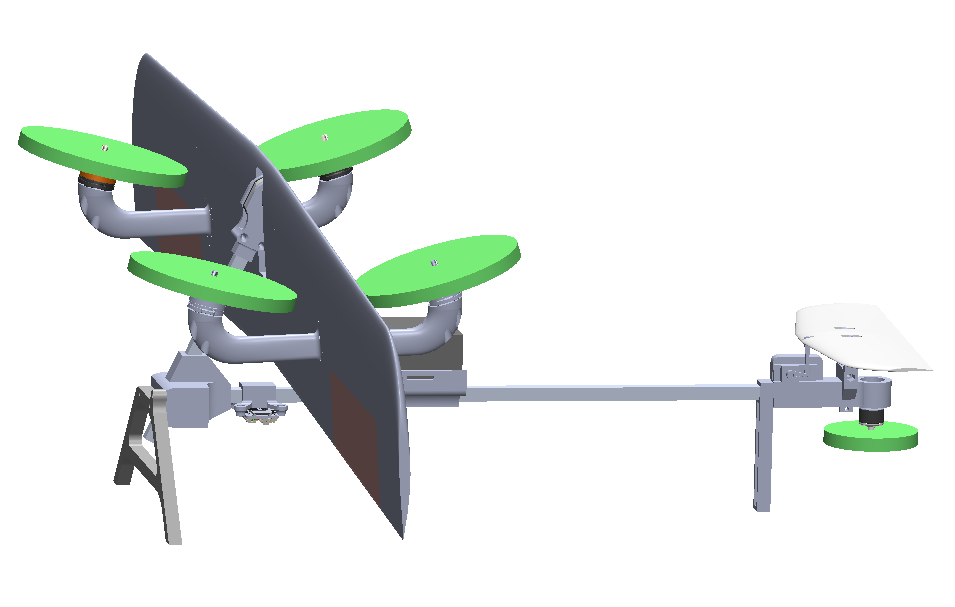
\includegraphics[width=1\columnwidth,angle=0]{picture/colibriH.jpg}
%     \caption{The Colibri convertible UAV, H version. }
%     \label{fig:colibri_h}
% \end{figure}

% L'architecture en H offre un actionnement important 

% \begin{figure}[h]
% \centering
%     \includegraphics[width=1\columnwidth,angle=0]{picture/ColibriV2.png}
%     \caption{The Colibri convertible UAV, motor on the wing. }
%     \label{fig:colibriv2}
% \end{figure}

\begin{figure}[h]
\centering
    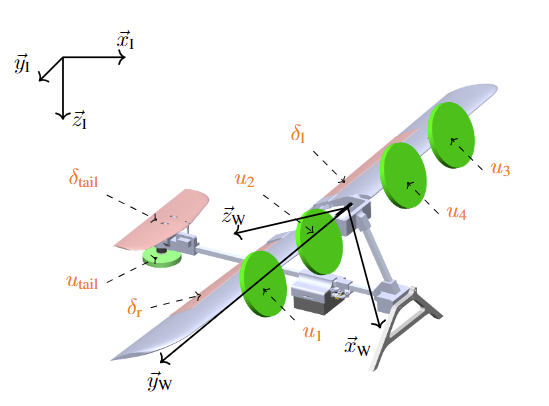
\includegraphics[width=1\columnwidth,angle=0,trim={0 0 0 0.5cm},clip]{figures/wold_body.png}
    \caption{Inertial (I) and wing (W) reference frames and the Colibri architecture. }
    \label{fig:world_body}
\end{figure}
% \todo{he reference frames could be introduced
% and detailed at the beginning of the section}

Some of the characteristic dimensions are shown in Table~\ref{tab:pars}. Note that the motors are positioned symmetrically on the wing, which means that the position can be described by focusing on one side. 
\begin{table}[ht]
  \centering
    \begin{tabular}{|l|c|c|}
      \hline
      \multicolumn{1}{|c|}{Parameter} & Value & Units  \\
      \hline
      $m_{\text{W}}$ (wing mass)  & 0.53& \SI{}{\kilogram} \\
      \hline
      $m_{\text{F}}$ (fuselage mass)  & 1.17& \SI{}{\kilogram} \\
      \hline
    %   $b$ (wingspan)  & 1.17 & \SI{}{\meter} \\
    %   \hline
    %   $c$ (aerodynamic cord)  & 0.150 & \SI{}{\meter} \\
    %   \hline
    %   $S$ (wing area) & 0.1537 & \SI{}{\square\meter}\\
    %   \hline
    %   $S_{\text{wet}}$ (wet area) & 0.0813 & \SI{}{\square\meter}\\
    %   \hline
    %   $S_{\text{p}}$ (propeller area) & 0.0182 & \SI{}{\square\meter}\\
    %   \hline
      $J_{\text{W}}=diag(J_{x}^{\text{W}}, J_{y}^{\text{W}}, J_{z}^{\text{W}})$ & \!\! $\diag(0.1677,0.0052,0.1634)$\!\! & \SI{}{\kilogram\square\meter}\\
      \hline
      $J_{\text{F}}=diag(J_{x}^{\text{F}}, J_{y}^{\text{F}}, J_{z}^{\text{F}})$ & \!\! $\diag(0.0191,0.0161,0.0343)$\!\! & \SI{}{\kilogram\square\meter}\\
      \hline
      $k_{\text{f}}$ (propeller thrust coeff.) & 1.7800e-8 & \SI{}{\kilogram\meter}\\
      \hline
    %   $k_{\text{m}}$(propeller torque coeff.) & 2.1065e-10 & \SI{}{\kilogram\square\meter}\\
    %   \hline
    %   $p_{z}^{int}$ (propeller $z$ location) & 0.037 & \SI{}{\meter}\\
    %   \hline
    %   $p_{y}^{int}$ (propeller $y$ location) & 0.145 & \SI{}{\meter}\\
    %   \hline
    %   $p_{z}^{ext}$ (propeller $z$ location) & 0.028 & \SI{}{\meter}\\
    %   \hline
    %   $p_{y}^{ext}$ (propeller $y$ location) & 0.325 & \SI{}{\meter}\\
    %   \hline
    %   $\xi_{\text{f}}$ (elevons lift coeff.) & 0.2 & --\\
    %   \hline
    %   $\xi_{\text{m}}$ (elevons torque coeff.) & 1.4 & --\\
    %   \hline
    %   $\rho$ (air density) & 1.225 & \SI{}{\kilogram\per\cubic\meter}\\
    %   \hline
    %   $C_{\text{d0}}$ (drag coeff.) & 0.1644 & --\\
    %   \hline
    %   $C_{\text{l0}}$ (lift coeff.) & 5.4001 & --\\
    %   \hline
       $d_{\text{M}O_{\text{W}}}$  & $[0.383,0,-0.167]^\top$ & \SI{}{\meter}\\
      \hline
       $d_{\text{G}O_{\text{W}}}$  & $[0.052,0,-0.171]^\top$ & \SI{}{\meter}\\
      \hline
    \end{tabular}
    \caption{\label{tab:pars} Numerical parameters of the Colibri model.}
\end{table}

% \todo{There is no derived process or explanation provided for
% the M matrix, A, Q matrix, etc. In Equation 1, both Q and B
% are matrices and do not include the location x. Where are
% the state variables located?}
The modelling is based on the results of \cite[Section 2.15]{udwadia-phohomsiri}. The algorithm for computing matrices $M$, $A$, $Q$ and $B$ is in \cite{udwadia-schutte}, which provides us the equations of motion of a constrained multibody system: 
\begin{align}
\label{eq:udwadia}
    \ddot{x} = \hat{M}^{\dag} \begin{bmatrix} Q \\ B \end{bmatrix}  = \begin{bmatrix} (I - A^{\dag}A)M \\ A \end{bmatrix}^{\dag} \begin{bmatrix} Q \\ B \end{bmatrix}
\end{align}
whose expression is valid as long as $\hat{M}$ has full rank and where $A$, $M$, $Q$ and $B$ are described next.\\
\begin{figure}[h]
\centering
    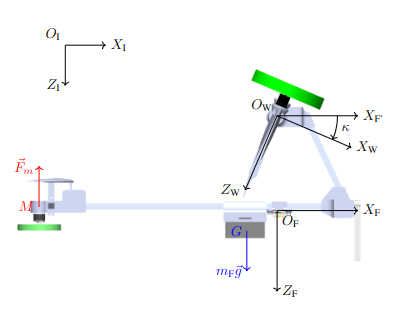
\includegraphics[width=1\columnwidth,angle=0,trim={0 0 0 0.5cm},clip]{figures/fram_side_colibri.png}
    \caption{Inertial (I), fuselage (F) and wing (W) reference frames and forces acting on the Colibri UAV.}
    \label{fig:colibri_frame_side}
\end{figure}
We will use quaternions $q = \left [ \eta ~ \epsilon^\top \right]^\top  \in {\mathbb S}^3:=\{ q\in \real^4: |q| = 1\}$ to represent the orientations of the two bodies.  The ensuing rotation matrix $R(q) \in SO(3): = \{R\in \real^{3\times 3}: \; 
 R^\top R = I, \det (R)=1\}$ is uniquely defined as 
$R(q) := I +2\eta \skewsym{\epsilon} + 2\skewsym{\epsilon}^{2} = [R_{1}~R_{2}~R_{3}]$. \\
According to Figure \ref{fig:world_body} and \ref{fig:colibri_frame_side}, define the vectors $p_{\text{F}} = \overrightarrow{O_{\text{I}} O_{\text{F}}} $, $p_{\text{W}} = \overrightarrow{O_{\text{I}} O_{\text{W}}} $, $d_{\text{FW}} = \overrightarrow{O_{\text{F}} O_{\text{W}}} $ satisfying $d_{\text{FW}} = p_{\text{W}} - p_{\text{F}}$ and $d_{\text{M}O_{\text{W}}} = \overrightarrow{\text{M} O_{\text{W}} }$, $d_{\text{G}O_{\text{W}}} = \overrightarrow{\text{G} O_{\text{W}} }$.

The overall state vector is $(x,v) \in \real^{28}$ with $x=(p_{\text{W}},~q_{\text{W}},~p_{\text{F}},~q_{\text{F}}) \in \real^{14}$ and $v=(v_{\text{W}},~\dot{q}_{\text{W}},~v_{\text{F}},~\dot{q}_{\text{F}}) = (\dot{p}_{\text{W}},~\dot{q}_{\text{W}},~\dot{p}_{\text{F}},~\dot{q}_{\text{F}})=\dot{x} \in \real^{14}$, where $v_{\text{W}} = \dot{p}_{\text{W}} \in \real^{3}$ represents the linear velocity of the wing in the inertial reference frame, $\dot{q}_{\text{W}} \in \real^{4}$ is the derivative of the quaternion, $q_{\text{W}} \in \real^{4}$ representing the orientation of the wing, $v_{\text{F}} =p_{\text{F}} \in \real^{3}$ is the linear velocity of the fuselage in the inertial reference frame and $\dot{q}_{\text{F}} \in \real^{4}$ is the derivative of the quaternion $q_{\text{F}} \in \real^{4}$ representing the fuselage orientation. It can be seen that the state vector is not minimal. It should be noted that the angular velocity $\omega \in \real^{3}$ can be obtained from the quaternion derivative $\dot{q}$ using equation  \cite[equation (2.7)]{udwadia-schutte} recalled here: 
\begin{align*}
    \omega = H(q) \dot{q} 
\end{align*}
where $H(q) \in \real^{3\times4}$ is a matrix defined by $H(q) = 2\begin{bmatrix}-\epsilon & \eta I_{3} - \skewsym{\epsilon}\end{bmatrix}$.
For deriving the equations of motion, recalling that $R_{i}(q) \in \real^{3}, i = 1,2,3$ are the three columns of a rotation matrix associated with quaternion $q$, define matrices  $L_{\text{i}}^{\text{W}} \left( q_{\text{W}} \right) = \frac{\partial R_{i}}{\partial q}(q_{\text{W}}) \in \real^{3\times4}$, 
$L_{\text{i}}^{\text{F}} \left( q_{\text{F}} \right) = \frac{\partial R_{i}}{\partial q}(q_{\text{F}}) \in \real^{3\times4}$ and
$L_{O_{\text{F}}^{\text{W}}} = \sum_{i=1}^{3} d_{\text{FW}}(i) L_{\text{i}}^{\text{F}} (q_{\text{F}})$, $i \in {1,2,3}$, where $d_{\text{FW}}(i)$ denotes the i-th component of vector $d_{\text{FW}} = p_{\text{W}} - p_{\text{F}}$. Since $O_{\text{W}}$ is located at the wing's center of rotation, the distance $d_{\text{FW}}$ is a constant, since $O_{\text{W}}$ and $O_{\text{F}}$ can be assumed to belong to the same solid (the fuselage). We deduce, with homogeneity, $\dot{L}_{O_{\text{F}}^{\text{W}}} = \sum_{i=1}^{3} d_{\text{FW}}(i) L_{\text{i}}^{\text{F}} (\dot{q}_{\text{F}})$. With these definitions, select the matrices in (\ref{eq:udwadia}) as
\begin{align}
    M = \begin{bmatrix}
        m_{\text{W}} I_{3} & \mathbb{0}_{3 \times 4} & \mathbb{0}_{3} & \mathbb{0}_{3 \times 4}\\
        \mathbb{0}_{4 \times 3} & H_{\text{W}}^\top J_{\text{W}} H_{\text{W}} & \mathbb{0}_{4 \times 3} & \mathbb{0}_{4}\\
        \mathbb{0}_{3} & \mathbb{0}_{3 \times 4} & m_{\text{F}} I_{3} & \mathbb{0}_{3 \times 4} \\
        \mathbb{0}_{4 \times 3} & \mathbb{0}_{4 } & \mathbb{0}_{4 \times 3} & H_{\text{F}}^\top J_{\text{F}} H_{\text{F}}    \end{bmatrix}\in \real^{14\times14},
\end{align}
where we denoted $H_{\text{W}} = H(q_{\text{W}})$, $H_{\text{F}} = H(q_{\text{F}})$, and
\begin{align}
    Q = \begin{bmatrix}
            m_{\text{W}} g e_3 + R(q_{\text{W}}) F_{\text{b}}\\
            -2\dot{H}_{\text{W}}^\top J_{\text{W}} \dot{H}_{\text{W}} \dot{q}_{\text{W}} + H_{\text{W}}^\top M_{\text{W}}\\
            m_{\text{F}} g e_3 + R(q_{\text{F}}) F_{\text{F}}\\
            -2\dot{H}_{\text{F}}^\top J_{\text{F}} \dot{H}_{\text{F}} \dot{q}_{\text{F}} + H_{\text{F}}^\top M_{\text{F}}\\
        \end{bmatrix} \in \real^{14},
\end{align}
% \todo{Details of forces and moments generated while the wing
% transits its position should be given in detail as this is
% the key distinct feature of this aircraft.}
where $\dot{H}_{\text{W}}$ denote $H(\dot{q}_{\text{W}})$, coinciding with the time derivative of $H(q_{\text{W}})$ and $\dot{H}_{\text{F}}$ denote $H(\dot{q}_{\text{F}})$, coinciding with the time derivative of $H(q_{\text{F}})$. Moreover, $F_{\text{b}}$ and $M_{\text{b}}$ represent, respectively,  all the forces and moments acting on the wing. The expressions of $M$ and $Q$ are taken from  \cite[equations (45) and (57)]{G003374} where the $\phi$ theory is developed, a parametrisation that allows the classical angles of incidence and sideslip to be subtracted and the hover singularity to be avoided. For lack of space, they will not be more detailed. Finally, $F_{\text{F}} =  F_{m}$ et $M_{\text{F}}$ represent respectively the set of non-gravitational forces and moments acting on the fuselage expressed in the frame $O_{\text{W}}$. In particular, $F_{m} = - k_{f} {u_{\text{tail}}}^{2}$ is the force generated by the motor located at the tail of the fuselage and $u_{\text{tail}}$ is the motor rotation speed, while
\begin{align}
    M_{\text{F}} =  m_{\text{F}} g e_3 \times d_{\text{G}O_{\text{W}}} + F_{m} \times d_{\text{M}O_{\text{W}}},
\end{align}
where $d_{\text{M}O_{\text{W}}}$ is the distance between the motor location and the center of rotation and $d_{\text{G}O_{\text{W}}}$ is the distance between the location of the fuselage's center of gravity and the center of rotation.

The set of constraints associated with the nonminimality or the state $(x,v)$ and by the pivot connection between the two bodies is given by:
\begin{align}
    \label{eq:contraintes}
    \left\{
    \begin{aligned}
    &\varphi_{1} \coloneqq q_{\text{W}}^\top q_{\text{W}} - 1 = 0\\
    &\varphi_{2} \coloneqq q_{\text{F}}^\top q_{\text{F}} - 1 = 0\\
    &\varphi_{3} \coloneqq R_{2}(q_{\text{W}})^\top R_{3}(q_{\text{F}}) = 0\\
    &\varphi_{4} \coloneqq R_{2}(q_{\text{W}})^\top R_{1}(q_{\text{F}}) = 0\\
    &\varphi_{5} \coloneqq p_{\text{F}} + d_{\text{FA}} + p_{\text{W}} = 0
    \end{aligned}
    \right.
\end{align}

The first two constraints impose the unit norm of the quaternions $q_{\text{F}}$ and $q_{\text{W}}$.
The third and fourth constraints are related to a moving pivot constraint, i.e. the orthogonality of two vectors is imposed. The last one is a positional constraint so that the point of the centre of rotation belonging to the wing coincides with the point defined in the fuselage. This constraint is based on a three-dimensional geometric closure.\\
It is more convenient to express the set of constraints as a stable dynamical system converging to zero, so we convert each one of the constraints in the form:
\begin{align}
    \ddot{\varphi_{i}} + \delta_{1} \dot{\varphi_{i}}  + \delta_{2} \varphi_{i} = 0, i \in {1,2,3,4,5},
\end{align}
with the selections $(\delta_{1}, \delta_{2}) = (0.5,~8)$ being the coefficients of a stable polynomial, so that, regardless of the selection $\varphi_{i}(0) = 0$, we have $\lim\limits_{t \to \infty} \varphi_{i}(t) = 0$. By differentiating constraints (\ref{eq:contraintes}) twice and factoring them out in the form $ A(x,\dot{x}) \ddot{x} = B(x,\dot{x})$, we obtain the expression of $A(x,\dot{x})$ reported in equation  (\ref{eq:A_contraint}) and $B(x,\dot{x})$ reported in the equation  (\ref{eq:b_contraint}) at the start of the next page.

\begin{align}
\label{eq:A_contraint}
    A = \begin{bmatrix}
            \mathbb{0}_{1 \times 3} & q_{\text{W}}^\top & \mathbb{0}_{1 \times 3} & \mathbb{0}_{1 \times 4}\\
            \mathbb{0}_{1 \times 3} & \mathbb{0}_{1 \times 4} & \mathbb{0}_{1 \times 3} & q_{\text{F}}^\top\\
            \mathbb{0}_{1 \times 3} & R_{3}(q_{\text{F}})^\top L_{2}^{\text{W}}( q_{\text{W}} ) & \mathbb{0}_{1 \times 3} & R_{2}(q_{\text{W}})^\top L_{3}^{\text{F}}( q_{\text{F}} ) \\
            \mathbb{0}_{1 \times 3} & R_{1}(q_{\text{F}})^\top L_{2}^{\text{W}}( q_{\text{W}} ) & \mathbb{0}_{1 \times 3} & R_{2}(q_{\text{W}})^\top L_{3}^{\text{F}}( q_{\text{F}} ) \\
            \mathbb{I}_{3} & L_{O_{\text{F}}^{\text{W}}} & -\mathbb{I}_{3} & \mathbb{0}_{3 \times 4}
        \end{bmatrix}
\end{align}

The simulation of a drone remains complex, as it is naturally unstable. We have chosen to use the control law proposed in \cite{SANSOUACA} extended to 6 DOF dynamics to stabilize the system. This PI-based control stabilises the wing. Another control law based on a proportional-derivative feedback stabilises the fuselage to keep it horizontal. The closed-loop simulation results are shown in Figure \ref{fig:sim_colibri}.
\begin{figure}[!h]
\centering
    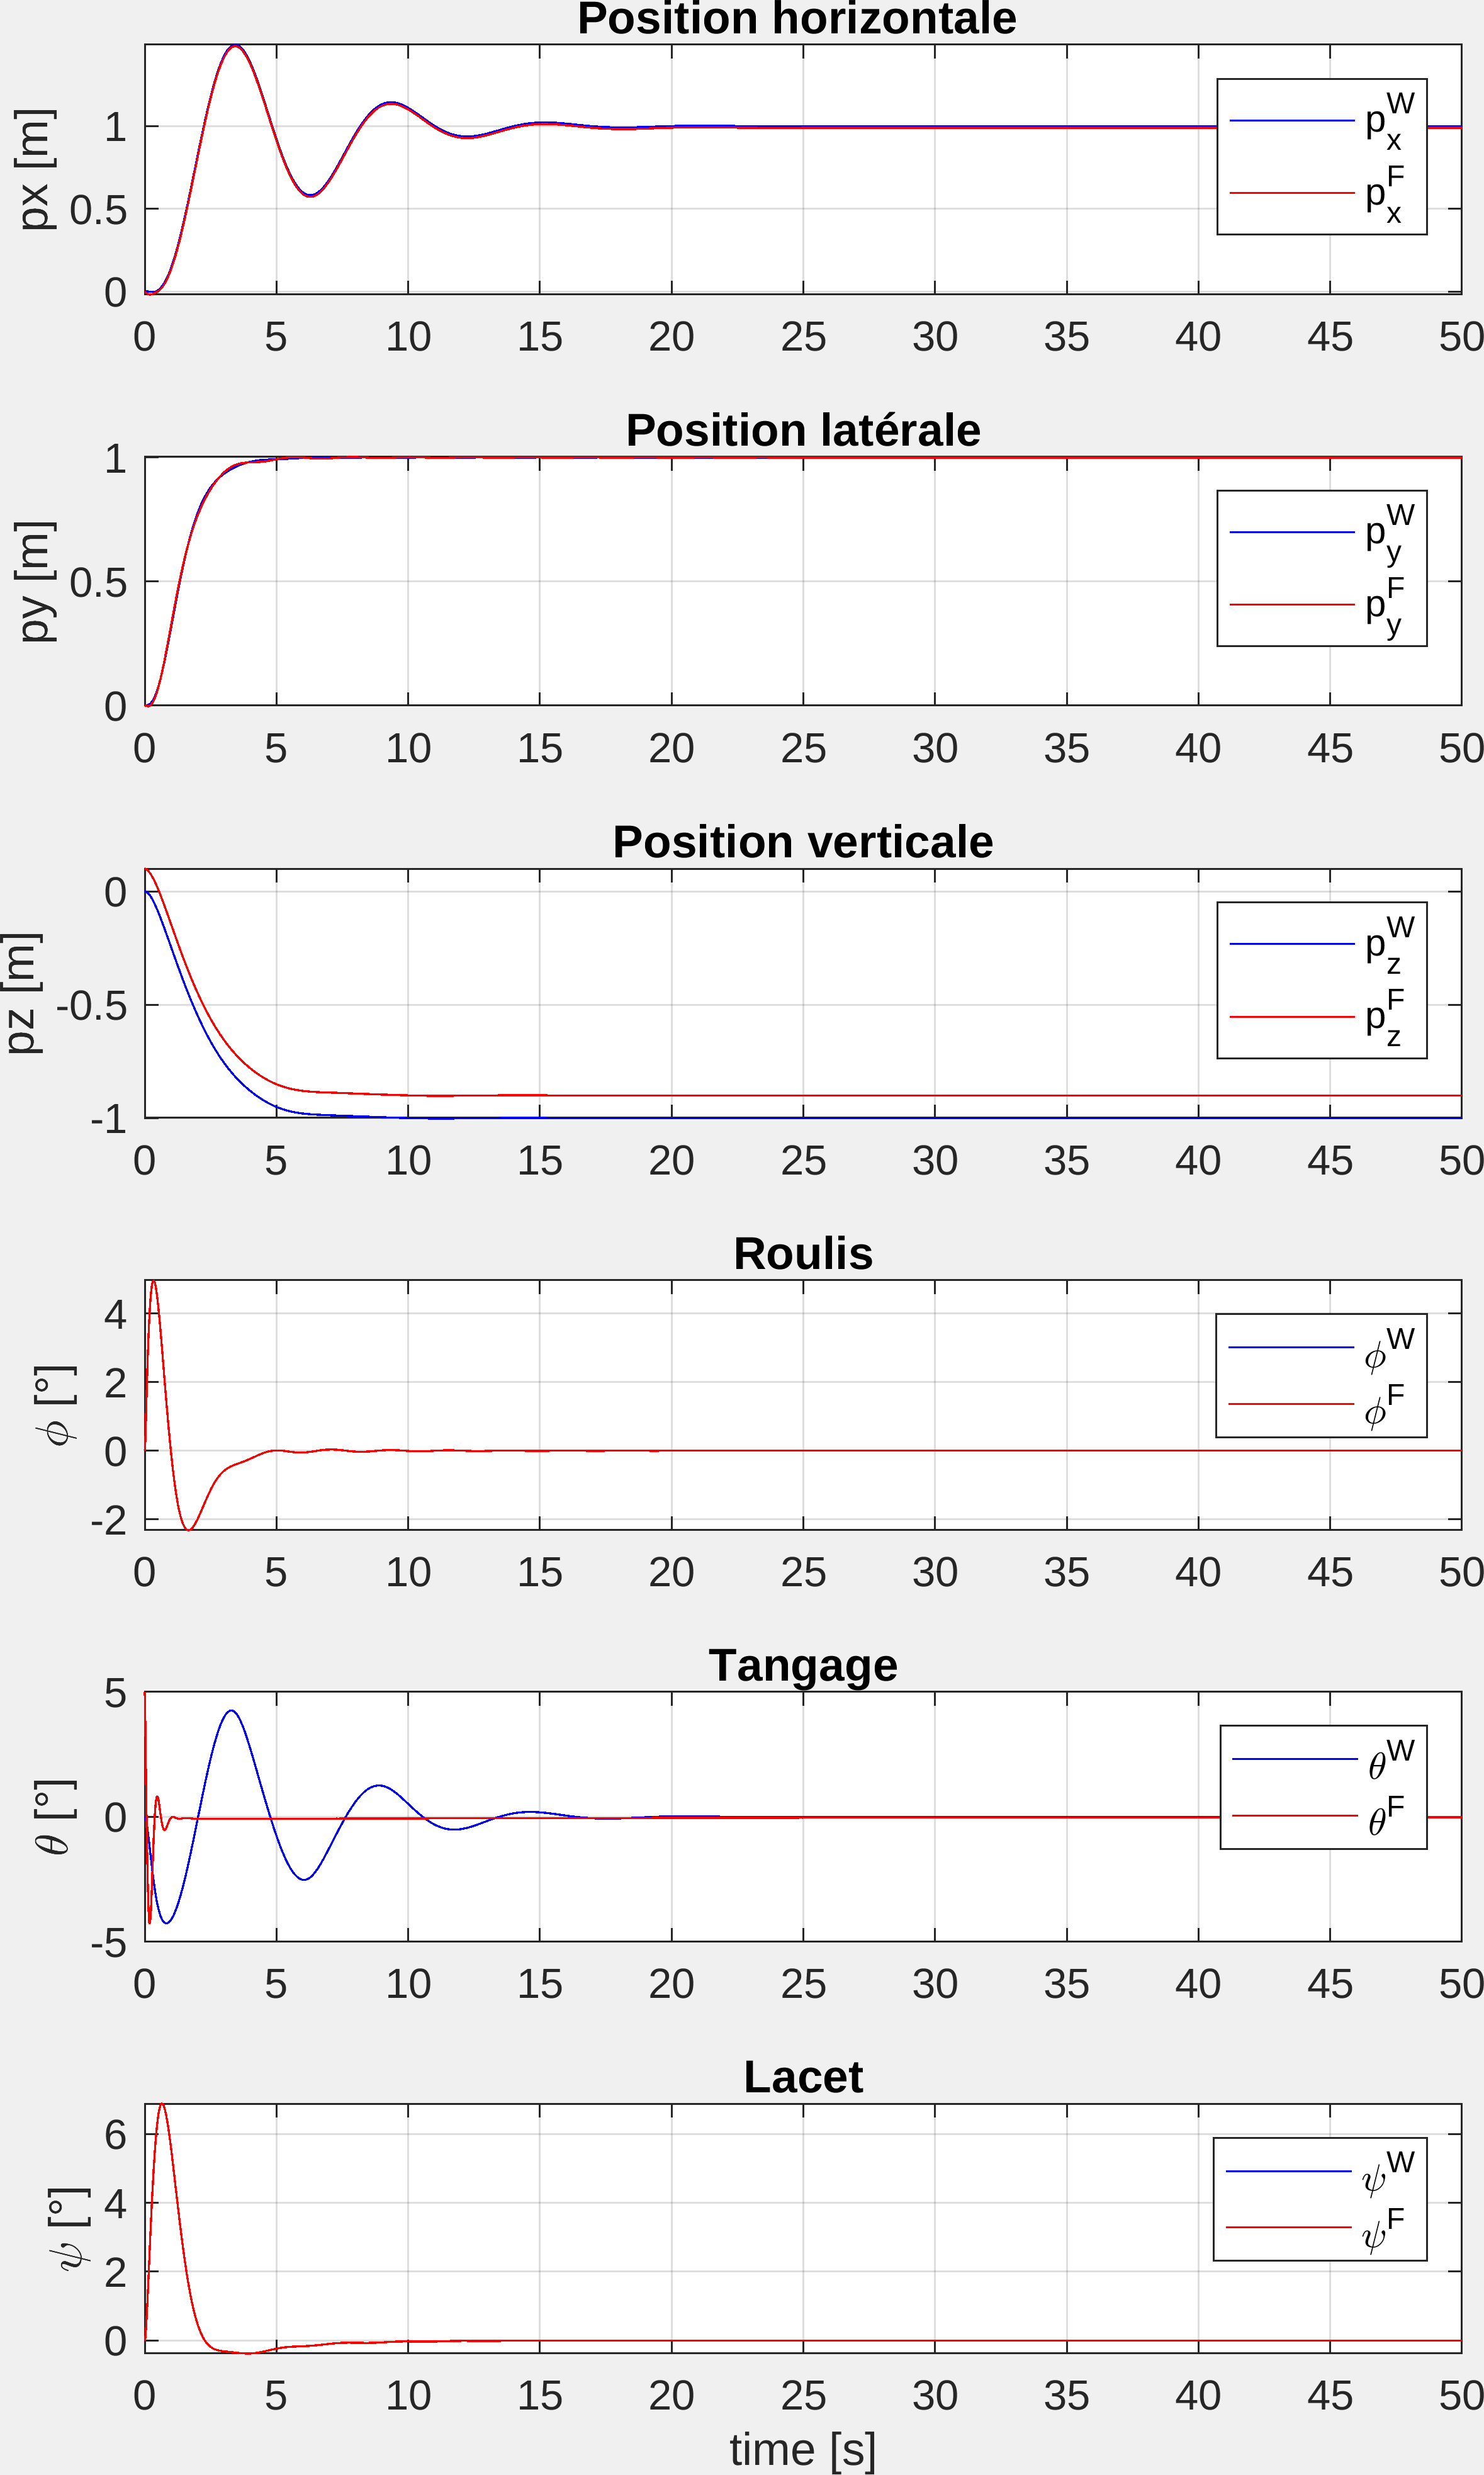
\includegraphics[width=1\columnwidth,angle=0]{figures/colibri_sim.png}
    \caption{Position and orientation simulation of the multi-body UAV Colibri in closed loop with a simple double-loop controller. }
    \label{fig:sim_colibri}
\end{figure}
Considering the degrees of freedom of the pivot link, the coupling between the two bodies is clearly visible from the lower three plots. Indeed, the roll and yaw angles $(\phi_{\text{F}}, \psi_{\text{F}})$ and $(\phi_{\text{W}}, \psi_{\text{W}})$ of the fuselage and wing coincide perfectly, while the pitch angles $(\theta{\text{F}}, \theta{\text{F}})$ are radically different.

\begin{figure*} [!h]
\begin{align}
\label{eq:b_contraint}
    B = \begin{bmatrix}
            -\delta_{1} q_{\text{W}}^\top \dot{q}_{\text{W}} - \frac{\delta_{2}}{2} (q_{\text{W}}^\top q_{\text{W}} -1) - \dot{q}_{\text{W}}^\top \dot{q}_{\text{W}} \\
            -\delta_{1} q_{\text{F}}^\top \dot{q}_{\text{F}} - \frac{\delta_{2}}{2} (q_{\text{F}}^\top q_{\text{F}} -1) - \dot{q}_{\text{F}}^\top \dot{q}_{\text{F}} \\
            -R_{3}(q_{\text{F}})^\top \dot{L}_{2}^{\text{W}}\dot{q}_{\text{W}} - R_{2}(q_{\text{W}})^\top \dot{L}_{3}^{\text{F}} \dot{q}_{\text{F}} - 2\dot{q}_{\text{W}}^\top {L_{2}^{\text{W}}}^\top L_{3}^{\text{F}} \dot{q}_{\text{F}} - \delta_{1}(R_{3}(q_{\text{F}})^\top L_{2}^{\text{W}}\dot{q}_{\text{W}} +  R_{2}(q_{\text{W}})^\top L_{3}^{\text{F}} \dot{q}_{\text{F}} ) - \delta_{2}\varphi_{3}\\
            -R_{1}(q_{\text{F}})^\top \dot{L}_{2}^{\text{W}}\dot{q}_{\text{W}} - R_{2}(q_{\text{W}})^\top \dot{L}_{1}^{\text{F}} \dot{q}_{\text{F}} - 2\dot{q}_{\text{W}}^\top {L_{2}^{\text{W}}}^\top L_{1}^{\text{F}} \dot{q}_{\text{F}} - \delta_{1}(R_{1}(q_{\text{F}})^\top L_{2}^{\text{W}}\dot{q}_{\text{W}} +  R_{2}(q_{\text{W}})^\top L_{1}^{\text{F}} \dot{q}_{\text{F}} ) - \delta_{2} \varphi_{4}\\
            \dot{L}_{O_{\text{F}}^{\text{W}}} \dot{q}_{\text{F}}  - \delta_{1}( v_{\text{W}} + \dot{L}_{O_{\text{F}}^{\text{W}}} \dot{q}_{\text{W}} - v_{\text{F}}) - \delta_{1}\varphi_{5}
        \end{bmatrix}
\end{align}
  \hrulefill\par
\end{figure*}




\section{State estimation}\label{sec:stateEst}
% \todo{Link to the modeling:  What is the connection between angular velocity
% estimation and the multibody dynamics derived in the paper?
% What are the advantages of the angular velocity estimator
% compared to existing technologies? It is difficult to
% discern the theoretical contribution to the angular
% velocity estimation part.}
In order to stabilise this two-body UAV system, it is necessary to know the position and orientation of the two bodies. Due to the pivot link between the wing and the fuselage, the difference between the orientation of the wing and the orientation of the fuselage is simply a rotation about the pitch axis of the wing. The two other orientations (roll and yaw) coincide. The position of the fuselage's centre of gravity can be deduced from the position of the wing's centre of gravity and the angle between the fuselage and the wing. This angle is measured by a quadrature rotary encoder (CUI Devices AMT22, Absolute Encoders, 12 bit, SPI), which returns a quantized angular measurement with a step size of \SI{0.09}{\degree}. Given this angular measurement, we discuss below the estimation of the speed information, so as to reconstruct the state of the UAV. 

\subsection{Sensors placement}
\label{subsec:sens_pos}
A first question pertains to the sensors placements: the IMU (accelerometer, gyroscope and magnetometer) can be installed on the fuselage or on the wing. 
Installing the IMU on the wing means that the measurements can be taken directly in the desired reference frame, but the measurements are noisier because the IMU is attached to the structure supporting the motors. Given the size of the wing, their flexibility can generate resonances and can perturb the measurements. 
%In addition, wiring the IMU is not easy as the cables must pass through the pivot link, which generates resistive torques.
Installing the IMU on the fuselage reduces vibrations, but means that the measurements must be transformed in the wing reference frame. The corresponding transformation can be computed from the rotary encoder measurement, providing the angle between the wing and the fuselage, and also from the measurements taken with the CAD software, providing precise information about the distances between the wing and fuselage frames. Our final choice is to attach the IMU to the fuselage. Another consideration is that the autopilot board, which already have an integrated IMU, is also supposed to be connected to the payload and other sensors attached to the fuselage. It is thus limiting the number of cables at the pivot point to the actuators commands and power supply.

\subsection{Angular speed estimation}
As explained above, we can measure the angle $\kappa \in \real$ between the wing and the fuselage using the rotary encoder. Then, to estimate the angular velocity we use the high-gain observer proposed in \cite{203613} (see also \cite{1032320} for the use of high-gain observers to estimate time derivatives). This method is preferable to a finite difference derivative, as the quantized information generated by the rotary encoder can result in bursts in the estimated angular velocity values.\\ 
Denote by $\kappa \in \real$ the measured position variable, by $\omega_{\kappa} := \dot \kappa  \in \real$ its derivative, to be estimated, and by $\xi = [\kappa,~\omega_{\kappa}]^\top \in \mathbb{R}^2$ their juxtaposition in a single vector. Denote also $\hat{\xi}$ the estimate of $\xi$ as follows:
%\todo{GH: il y a pas un peu de répétitions dans les notations ?}
%\xi = [\kappa,~\omega_{\kappa}]^\top \in \mathbb{R}^2, \quad 
\begin{align*}
    \hat{\xi} = [\hat{\kappa},~\hat{\omega}_{\kappa}]^\top \in \mathbb{R}^2.
\end{align*}
Following \cite{203613}, the estimator dynamics is given by
\begin{align}
\label{eq:high_dyn}
    \dot{\hat{\xi}} =  \begin{bmatrix}0 & 1 \\ 0 & 0 \end{bmatrix} \hat{\xi}+ \begin{bmatrix}\frac{k_{p}}{\epsilon_{\kappa}}  \\ \frac{k_{v}}{\epsilon_{\kappa}^{2}}  \end{bmatrix} (\kappa - \hat{\kappa}),
\end{align}
where $\kappa$ is the angular measurement recovering from the sensors, $k_{p}$ and $k_{v}$ are two positive scalars gains such that the characteristic equation $s^{2} + k_{v} s + k_{p} = 0$ has roots with negative real part. For our estimators, we have selected $k_{p} = 1$ and $k_{v} = 1.3$ so as to get a damping factor $\zeta = 0.65$ leading to a slightly underdamped response as a suitable trade-off between a fast rise time and a mildly oscillatory response. The high-gain scaling factor
$\epsilon_{\kappa}$ can be conveniently adjusted in order to obtain a trade-off between smoothing action (obtained by increasing $\epsilon_{\kappa}$) and reduction of the time lag
of the estimator (obtained by reducing $\epsilon_{\kappa}$). Moreover, the smoothing action of the proposed approach mitigates the effect of the quantized position measurements. We have selected $\epsilon_{\kappa} = 0.05$ for our experiments. Figure \ref{fig:high_gain} shows the experimental results obtained after implementation of the high-gain filter (\ref{eq:high_dyn}) in the case of a flight generating high-amplitude angular oscillations.
\begin{figure}[h]
\centering
    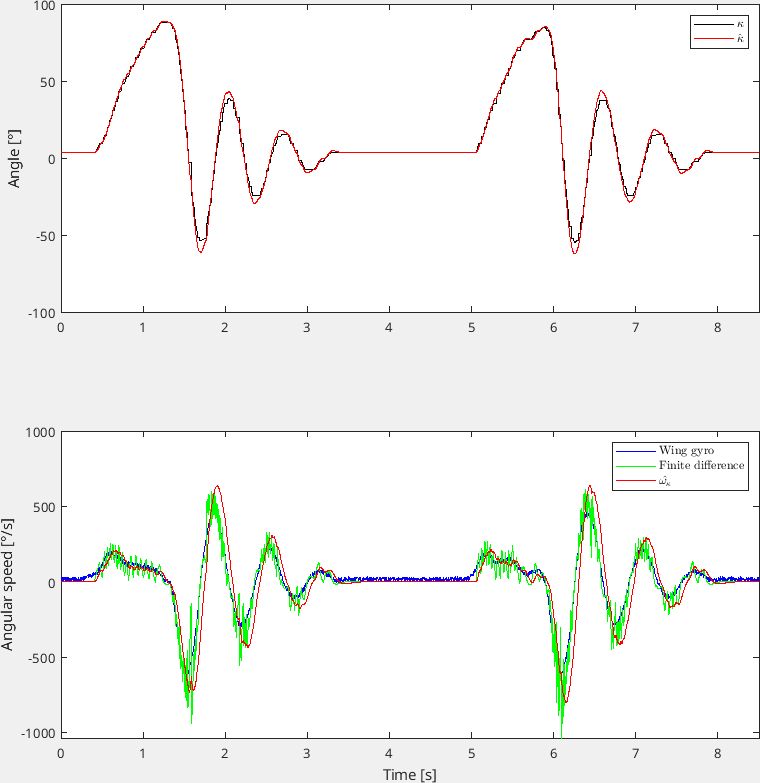
\includegraphics[width=1\columnwidth,angle=0]{figures/highGainFilter.png}
    \caption{Angular position measurement (black,top plot), wing gyro velocity measurement (blue,bottom plot), finite difference velocity estimation (green, bottom plot) and high-gain estimates (red curves)}
    \label{fig:high_gain}
\end{figure}
%\todo{GH: c'est pas très lisible comme figure}
We carried out differentiation by finite difference (in green) in post-treatment to compare the results. Due to the quantized nature of the rotary encoder, we observe that the angular velocity obtained by finite difference is very noisy. We can see that the high-gain filter makes it possible to estimate the angular velocity more accurately (in red), albeit with a slight delay. Thanks to the addition of an extra IMU on the wing in a specific flight test, it is possible to compare the velocity estimate with the wing's gyroscope (MPU9250) measurements, visible on the bottom graph of Figure \ref{fig:high_gain} (blue trace). We can see that the gyroscope readings are somewhat noisy, due in particular to the vibrations generated by the motors.  %\todo{GH: ref à la figure est trop tard par rapport au texte}
\\
In order to perform the necessary transformation among the reference frames, define the quaternion $q_{\hat{\kappa}} \in {\mathbb S}^3$ as follows:
\begin{align}
\label{eq:rot_quat}
    q_{\hat{\kappa}} =  \left [\cos\left(\frac{\hat{\kappa}}{2}\right) ~ 0 ~ \sin\left(\frac{\hat{\kappa}}{2}\right) ~ 0 \right]^\top
\end{align}


\subsection{Wing state estimation}
Based on the estimated angle $\hat{\kappa}$ and the estimated angular velocity $\hat{\omega}_{\kappa}$, it is possible to transform the measurements from the fuselage to the wing frame. All the sensors are installed on the autopilot board, which is itself attached to the fuselage. However, as mention in introduction, we want to use INDI to stabilize the wing. So this control law requires the state information in the wing reference frame, where all the forces are applied (aerodynamic and traction).
Then, two viable solution are possible: perform the state estimation in the fuselage reference frame and rotate the estimation, using the estimate of the angle $\hat{\kappa}$, or rotate the raw measurements in advance to express them in the wing reference frame, and then perform the state estimation on the latter. 
Given the current architecture of the software in the Paparazzi\footnote{\url{https://github.com/enacuavlab/paparazzi/tree/rot_state_est}} system, it is cumbersome to have two joint state estimation structures, so it is difficult to implement the first solution, where the controller directly retrieves the current state estimation. For this reason, we have chosen to estimate the state of the wing from data measured on the fuselage. To this end, we detail below the coordinate transformation for the three sensors: gyroscope, accelerometer and magnetometer. \\
\indent For the gyroscope-based angular rate measurements, we may compute the angular velocity of the wing expressed in the wing frame as
\begin{align}
    \label{eq:gyro_deplacement}
    \omega_{\text{W}} = R(q_{\hat{\kappa}}) \left( \omega_{gyro}^{\text{F}} + \begin{bmatrix}
    0\\ \omega_{\kappa} \\ 0
    \end{bmatrix}  \right) 
\end{align}
where $\omega_{gyro}^{\text{F}}$ is the angular velocity measured by the gyro on the fuselage, expressed in the fuselage frame, $\hat{\omega}_{\kappa}$ is the estimated angular velocity of the wing relative to the fuselage, as per (\ref{eq:high_dyn}), and $q_{\hat{\kappa}}$ is the quaternion defined in (\ref{eq:rot_quat}).
Expression (\ref{eq:gyro_deplacement}) is similar to a composition of angular velocities and a reference frame transformation.\\
\indent For the acceleration measurement with the accelerometer, we may use the following relation
Expression (\ref{eq:accel_deplacement}) is obtained from the rate of change transport theorem \cite{brizard2004motion}, where we find the Euler acceleration term $\dot{\omega_{\text{F}}} \times d_{AF}$ and the centripetal acceleration term $\omega_{\text{F}} \times ( \omega_{\text{F}} \times  d_{AF})$. Coriolis Acceleration $2\omega_{\text{F}} \times \frac{d (d_{\text{FW}})}{d t}\Bigr|_{O_{\text{F}}}$ and the rate of acceleration $\frac{d^{2} (d_{\text{FW}})}{d^{2} t}\Bigr|_{O_{\text{F}}}$ are zero because $d_{\text{FW}}$ is contant.
\begin{align}
    \label{eq:accel_deplacement}
    a_{\text{W}} = R(q_{\hat{\kappa}}) \left( a_{acc}^{F} + \dot{\omega}_{gyro}^{F} \times d_{\text{FW}} + \omega_{gyro}^{F} \times ( \omega_{gyro}^{F} \times  d_{\text{FW}}) \right) 
\end{align}
where $a_{acc}^{F} \in \real^{3}$ is the acceleration measured by the accelerometer on the fuselage, expressed in the fuselage frame and $\omega_{gyro}^{F}$, the angular velocity of the fuselage, same as the equation (\ref{eq:gyro_deplacement}). The angular acceleration $\dot{\omega}_{gyro}^{F}$ in (\ref{eq:accel_deplacement}) is computed by a finite difference.\\
\indent For the magnetometer measurements, we have
\begin{align}
    \label{eq:mag_deplacement}
    E_{\text{W}} = R(q_{\hat{\kappa}}) E_{mag}
\end{align}
where $E_{mag} \in \real^{3}$ is the magnetometer output, expressed in the fuselage frame and  $ E_{\text{W}} \in \real^{3}$ is the computed measurement expressed in the wing frame.\\
\indent To obtain the wing state estimate, we use a sensor measurement fusion algorithm: extended Kalman filter\footnote{\url{https://github.com/PX4/PX4-ECL/tree/master}} (EKF) which provide an estimate of the following states: $p_{\text{W}}$, $v_{\text{W}}$, $q_{\text{W}}$ from measurements transformed in the wing reference frame $\omega_{\text{W}}$ (eq. (\ref{eq:gyro_deplacement})), $a_{\text{W}}$ (eq. (\ref{eq:accel_deplacement})), $E_{\text{W}}$ (eq. (\ref{eq:mag_deplacement})) and external vision system pose data, which provides a precise measurement of the drone's position $p_{\text{W}}$ and speed $v_{\text{W}}$ in the inertial reference frame (I).

\subsection{Fuselage orientation estimation}
To determine the orientation of the fuselage, we may perform a composition between the quaternion representing the orientation of the wing $q_{\text{W}}$ result of EKF and the quaternion constructed from the filtered measurement of the rotary encoder $q_{\hat{\kappa}}$ in (\ref{eq:rot_quat}),
\begin{align}
\label{eq:quat_fuselage}
    q_{\text{F}} = q_{\text{W}} \otimes q_{\hat{\kappa}}
\end{align}
where the operator $\otimes$ denotes the qaternion product. The knowledge of $q_{\text{F}}$ is needed to keep the fuselage perfectly horizontal. 









